\documentclass[tikz,border=5pt]{standalone}
\usepackage{amsmath}
\usetikzlibrary{arrows.meta,positioning,calc}

\begin{document}
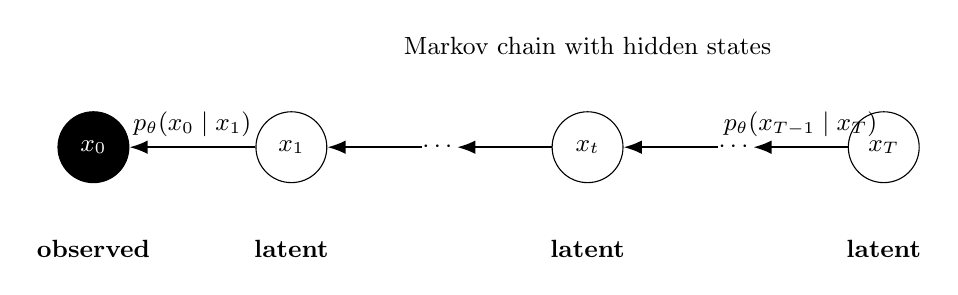
\begin{tikzpicture}[>=Latex, font=\small]
  % chain (reverse-direction graphical model)
  \node[draw, circle, fill=black, text=white, minimum size=9mm] (x0) {$x_0$};
  \node[draw, circle, minimum size=9mm, right=1.6cm of x0] (x1) {$x_1$};
  \node[inner sep=0pt, right=1.2cm of x1] (dots1) {$\cdots$};
  \node[draw, circle, minimum size=9mm, right=1.2cm of dots1] (xt) {$x_t$};
  \node[inner sep=0pt, right=1.2cm of xt] (dots2) {$\cdots$};
  \node[draw, circle, minimum size=9mm, right=1.2cm of dots2] (xT) {$x_T$};

  \draw[->, thick] (xT) -- node[above] {$p_\theta(x_{T-1}\mid x_T)$} (dots2);
  \draw[->, thick] (dots2) -- (xt);
  \draw[->, thick] (xt) -- (dots1);
  \draw[->, thick] (dots1) -- (x1);
  \draw[->, thick] (x1) -- node[above] {$p_\theta(x_0\mid x_1)$} (x0);

  % observation mark
  \node[below=0.6cm of x0] {\textbf{observed}};
  \node[below=0.6cm of x1] {\textbf{latent}};
  \node[below=0.6cm of xt] {\textbf{latent}};
  \node[below=0.6cm of xT] {\textbf{latent}};

  \node[above=0.6cm of xt] {Markov chain with hidden states};
\end{tikzpicture}
\end{document}



